\documentclass[11pt]{report}
\usepackage[utf8]{inputenc}
 \usepackage{listings}
 \usepackage{color}
 \usepackage{fancyhdr}
 \usepackage{graphicx}
\pagestyle{fancy}

 \lhead{Geoffrey PERRIN \\ Océane DUBOIS}
 \rhead{MI01 - TP03 : VHDL séquentiel temporisé}
 \rfoot{}



\definecolor{dkgreen}{rgb}{0,0.6,0}
\definecolor{gray}{rgb}{0.5,0.5,0.5}
\definecolor{mauve}{rgb}{0.58,0,0.82}

\lstset{frame=tb,
  language=vhdl,
  aboveskip=3mm,
  belowskip=3mm,
  showstringspaces=false,
  columns=flexible,
  basicstyle={\small\ttfamily},
  numbers=none,
  numberstyle=\tiny\color{gray},
  keywordstyle=\color{blue},
  commentstyle=\color{dkgreen},
  stringstyle=\color{mauve},
  breaklines=true,
  breakatwhitespace=true,
  tabsize=3
}


%Gummi|065|=)
\title{\textbf{TP02 - VHDL séquentiel temporisé}
\author{Geoffrey PERRIN \\ Océane DUBOIS\\}
\date{}}

\begin{document}

\maketitle

\newpage

\section{Exercice préliminaire}

Voici le code d'un diviseur de fréquence :
\begin{lstlisting}
entity blinker is
	port(Clk100MHz, PB_0 : in bit; --on utilise l'horloge 100MHz en signal d'entree
		LED_0 : out bit);
end blinker;

architecture Behavioral of blinker is
	alias reset is PB_0; --PB\_0 est defini comme le signal de reset
	signal clk_out : bit := '0'; -- signal d'horloge apres division
	constant clock_divisor : integer := 100000000; --constante de division pour un signal a 1Hz
	begin
		clock_divider : process(Clk100Mhz, reset)
		variable c : integer range 0 to clock_divisor - 1 := 0;
		begin
		if reset = '1' then -- si on declanche le reset on recommence le cycle de l'horloge a 0
			c := 0;
			clk_out <= '0';
		elsif Clk100MHz'event and Clk100MHz = '1' then --si le signal Clk100MHz est sur un front montant
			if c < (clock_divisor - 1) / 2 then --entre 0 et 0,5secondes on incremente c et on laisse la sortie a 0
				c := c + 1;
				clk_out <= '0';
			elsif c = (clock_divisor - 1) then -- lorsqu'on arrive a une seconde, on recommence le cycle a 0
				c := 0;
				clk_out <= '0';
			else -- sur la deuxieme partie du cycle (de 0,5 a 1seconde), on continue d'incrementer c et on passe la sortie a 1.
					c := c + 1;
			clk_out <= '1';
			end if;
		end if;
	end process;
-- Sortie sur la LED
LED_0 <= clk_out;
end Behavioral;
\end{lstlisting}

Dans ce code, on définit d'abord une entité "blinker", consituté de 2 ports d'entrée : Clk100MHz, PB\_0 et une sortie LED\_0.

Puis dans l'architecture, on définit un alias pour PB\_0 qui sera désomais appelé reset. On définit un nouveau signal de type bit, appelé clk\_out qui est initialisé à 0 qui sera le signal de sortie.  Et une constante de type entier nommé clock\_divisor initialisé à 100000000.

Puis on déclare un process donc la liste de signaux de sensibilité est composée des signaux Clk100Mhz et reset.C'est donc un reset asynchrone.

Dans le process si le reset est activé, on met la variable c à 0 et le signal clock\_out à 0. Si le signal Clk100MHz est sur un front montant et que la variable c est inferieur à (100000000-1)/2 =49999999,5 alors on incrémente la variable c et le signal clock\_out est mis à 0. Si c = 99999999 on met c à 0 et clv\_out à 0. Entre 49999999,5 et 99999999 on met la sortie à 1.
A la fin du process on égalise clk\_out sur LED\_0.

La LED\_0 est donc activée (à 1) à chaque cycle (de 1 entre 0,5 secondes et 1 seconde le reste du temps elle est à 0.

\begin{figure}[h]
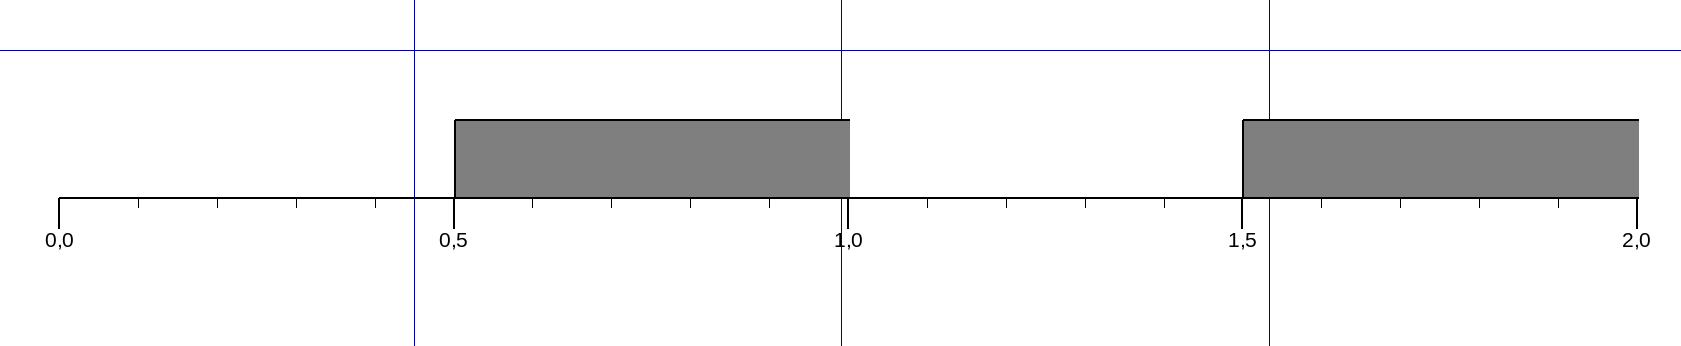
\includegraphics[width=10cm]{TP03-1.PNG}
\caption{Chronograme du fonctionnement du blinker}
\end{figure}


\section{Feu de circulation}

Dans cet exercices on cherchera à implémenter un contrôleur de circulation, permettant de réguler la circulation d'un croisement à 2 axes principaux.

Le feu rouge dure 10 secondes et le feu orange 2 secondes. Le feu vert doit donc durer 8 secondes. Puisqu'il faut que Trouge = Tvert + Torange.

La plus petite unité de temps utilisée est donc 2 secondes (Tsync), on  peut donc utiliser une fréquence d'horloge de f=1/Tsync=0,5Hz

On nomme les 2 axes A et B qui sont perpendiculaires. Lorsque le feu de l'axe A est au rouge, le feu de l'axe B doit être vert puis passer au orange. Puis le feu de l'axe B passe enfin au rouge, et le feu de l'axe A passe au vert puis 8 secondes plus tard au orange.

On peut réaliser cette modélisation en comportemental ou en structurel.

On choisi ici de modéliser les feu de circulation à l'aide d'un code en VHDL comportemental car cela nous semble plus simple d'inclure le blinker dans le code VHDL. En structurel nous aurions du créer une entité blinker qui aurait ensuite été utilisée dans le code VHDL des feux de circulation. 

On réalise un modélisation à partir d'un machine à états

\begin{figure}[h]
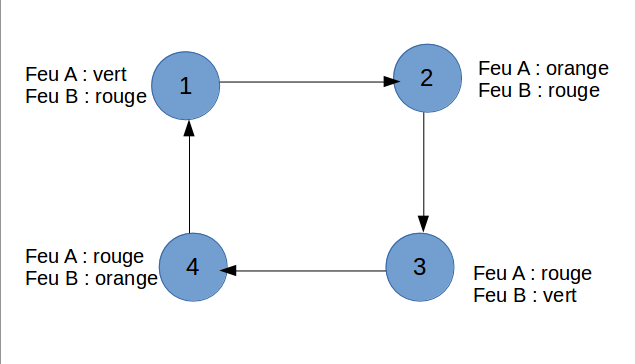
\includegraphics[width=12cm]{TP03-2.png}
\caption{Machine à état des feux}
\end{figure}

La machine reste dans l'état 1 pendant 8 secondes, puis dans l'état 2 pendant 2 secondes puis dans l'état 3 pendant 8 secondes et enfin dans l'état 4 pendant 2 secondes. 

Ainsi de 0 à 8 secondes, le feu A est vert et le feu B est au rouge, de 8 à 10 secondes, le feu A est orange et le feu B est rouge, de 10 à 18 secondes, le feu A est rouge et le feu B est vert et de 18 à 30 secondes, le feu A est rouge et le feu B est orange. A la fin, on recommence le cycle depuis le début. 


On utilisera dans le code VHDL des entiers pour différencier les couleurs de feu, soit la valeur 1 pour signaler un feu rouge, 2 pour le feu orange et 4 pour le feu vert.






// recopier le bon code VHDL
\subsection{Code VHDL}
\begin{lstlisting}
ENTITY feu IS
	PORT(Clk100MHz, PB_0 : INBIT;
		LED_3210, LED_7654 : OUT INTEGER RANGE 0 TO 4);
END feu

ARCHITECTURE Behavioural OF feu IS
alias reset is PB_0;
signal clk_out : bit := '0';
constant clock_divisor : integer := 100000000;
BEGIN
	clock_divider : PROCESS(Clk100Mhz, reset)
	variable c : integer range 0 to clock_divisor - 1 := 0;
		begin
		if reset = '1' then
			c := 0;
			clk_out <= '0';
		elsif Clk100MHz'event and Clk100MHz = '1' then

			if c < (clock_divisor - 1) / 2 then
				c := c + 1;
				clk_out <= '0';
			elsif c = (clock_divisor - 1) then
				c := 0;
				clk_out <= '0';
			else
			c := c + 1;
				clk_out <= '1';
			end if;

		end if;
		end process;

	process(clk_out)

	variable c : integer range 0 to 20; --temps total d'un cycle
	variable etat : integer range 0 to 3;
	variable feuA, feuB : integer range 0 to 4;

	begin
		if reset = '1' then
			c := 0;
			etat := 0;
		elsif clk_out'Event and clk_out = '1' then
			if c < 8 then
				c := c + 1;
				etat := 0;
			elsif c < 10 then
				c := c + 1;
				etat := 1;
				elsif c < 18 then
				c := c + 1;
				etat := 2;
			elsif c < 20 then
				c := c + 1;
				etat := 3;
			end if;
			if c = 20 then
			   c := 0;
			end if;
		end if;

		case etat is
			when 0 => feuA <= 1; feuB <= 3; --le feu de l'axe A est vert et le feu de l'axe B est rouge
			when 1 => feu1 <= 2; feuB <= 3; --le feu de l'axe A est orange, le feu de l'axe B est rouge
			when 2 => feu1 <= 3; feuB <= 1; --le feu de l'axe A est rouge, le feu de l'axe B est vert
			when 3 => feu1 <= 3; feuB <= 2; --le feu de l'axe A est rouge et le feu de l'axe B est orange
			when others => feu1 <= 1; feuB <= 4;
		end case;

	end process;

	LED_3210 <= feuA;
	LED_7654 <= feuB;

	END Behavioural;


\end{lstlisting}

Sachant que le signal d'entrée du deuxième process est clk\_out et qu'il change d'état toutes les seconde, nous avons décidé de créer un compteur de temps, modélisé par la variable c, qui permet d'incrémenter la variable d'état toutes les 8 puis 2 secondes, plutôt que de faire une machine à 20 états différents.

Pour le reset nous avons défini le comportement du reset pour chacun des 4 états de la machine, afin d'essayer d'avoir le reset le plus sécurisé possible pour les automobiliste. 

Ainsi l'état de reset est défini ainsi : feu A au vert et feu B au rouge. 

Ainsi dans l'état 0 (feu A au vert et feu B au rouge), si on appuie sur le reset, on remet le compteur à 0 et on reste dans cet état.

Dans l'état 1 (le feu A est orange et le feu B est au rouge), si on appuie sur le reset on peut directement repasser dans l'état 0 aussi, car passer du orange vers le vert n'est, pour nous, pas un dangers pour les automobilistes.

Dans l'état 2 (le feu A est rouge et le feu B est vert), si on appuie sur reset, il faut passer le feu B au orange pendant 2 secondes puis ensuite passer au rouge et passer le feu A au vert. Cette séquence d'instruction correspond à celle qui se passe lorsqu'on est dans l'état 3 et qu'on repasse à l'état 0.

Dans l'état 3 (le feu A est au rouge et le feu B est au orange), si on appuie sur le reset il ne se passe rien, car on souhaite finir normalement le cyle et repasser ensuite à l'état 0, comme prévu normalement dans le code VHDL. 

\begin{figure}[h]
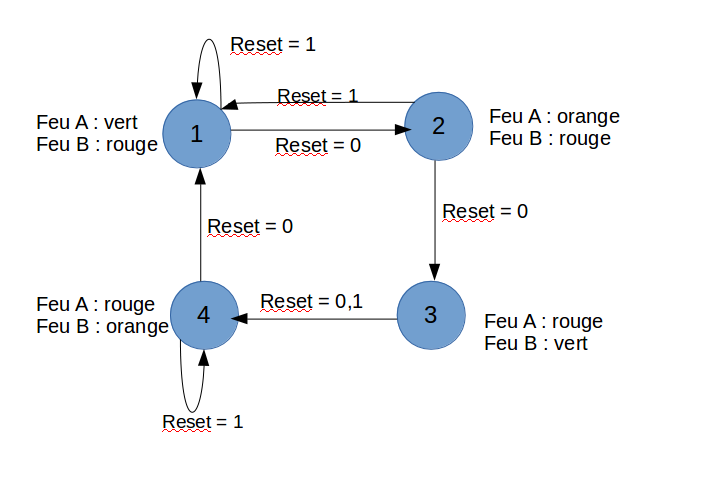
\includegraphics[width=10cm]{TP03-3.png}
\caption{Machine à état des feu avec reset}
\end{figure}



METTRE LE CODE AVEC LE RESET !

\section{Prise en compte d'un capteur de voiture}


Dans cet exercice on doit toujours réaliser un feu de voiture, mais cette fois-ci en considérant la présence d'un capteur de véhicule qui permet de savoir si il y a un véhicule sur l'axe ou non, si il n'y en a pas, on peut laisser le feu du deuxième axe vert. On ne prendra pas le reset en compte pour le moment.

Les signaux utilisés pour symboliser les capteurs de véhicules sont PB\_2 et PB\_3.

On définit donc les séquences comme suivant :
\begin{itemize}
	\item S'il n'y a pas de véhicules sur l'axe A, laisser le feu au vert sur l'axe B.
	\item Si un véhicule arrive sur l'axe A, le feu de l'axe B doit passer au orange, tout en ayant respecté les 8 secondes de feu vert sur l'axe A
	\item Ces comportements sont valable pour le feu de l'axe B. 

\end{itemize}

On décide donc, de définir les 4 états de notre machine à état ainsi :
\begin{itemize}
\item Dans l'état 1, si on detecte une voiture avec le capteur A mais aucune voiture avec le capteur B, on reboucle sur ce même état. Dans toutes les autres configurations de capteurs (ex : CapteurA=1 et CapteurB=1), on passe à l'état 2 lorsque c=8.
\item Dans l'état 2, on ne s'occupe pas des capteurs de voitures, dans tous les cas on passe à l'état 3.
\item Dans l'état 3, si on detecte une voiture avec le capteur B mais aucune voiture avec le capteur A, on reboucle sur cet état. Pour toutes les autres configurations, lorsque c est égale à 18 on passe à l'état 4.
\item Dans l'état 4, quelque soit la configuration des capteurs on passe à l'état 1 lorsque c=20.


\end{itemize}






\subsection{Code VHDL}

Le code VHDL que nous avons écrit a partir de cette nouvelle machine à état est le suivant : 

\begin{lstlisting}
	process(clk_out)

	variable c : integer range 0 to 20; --temps total d'un cycle
	variable etat : integer range 0 to 3;
	variable feuA, feuB : integer range 0 to 4;

	begin
		if reset = '1' then
			c := 0;
			etat := 0;
		else if clk_out'Event and clk_out = '1' then
			if (PB_3 = 1 and etat = 0) or (PB_2 = 1 and etat = 2) or (PB_2 = 1 and PB_3 = 1) then
				if c < 8 then
					c := c + 1;
					etat := 0;
				elsif c < 10 then
					c := c + 1;
					etat := 1;
				elsif c < 18 then
					c := c + 1;
					etat := 2;
				elsif c < 20 then
					c := c + 1;
					etat := 3;
				end if;
				if c = 20 then
				   c := 0;
				end if;
			end if;
		end if;

		case etat is
			when 0 => feuA <= 1; feuB <= 3;-- le feu de l'axe A est vert et le feu de l'axe B est rouge
			when 1 => feu1 <= 2; feuB <= 3;--le feu de l'axe A est orange, le feu de l'axe B est rouge
			when 2 => feu1 <= 3; feuB <= 1;--le feu de l'axe A est rouge, le feu de l'axe B est vert
			when 3 => feu1 <= 3; feuB <= 2; --le feu de l'axe A est rouge et le feu de l'axe B est orange
			when others => feu1 <= 1; feuB <= 4;
		end case;

	end process;

	LED_3210 <= feuA;
	LED_7654 <= feuB;

	END Behavioural;
  \end{lstlisting}
  
  \subsection{Synthèse}
  
  
  \subsection{Avec le reset}
  
  

\end{document}
